\chapter{Secure Shared Folder}\label{ch:ssf}

In this chapter, we describe in detail the Secure Shared Folder (SSF) scheme (\cref{sc:SSF-scheme}) and its implementation.
We detail the cryptographic implementation and usages of supporting
libraries, as well as their implications in terms of runtime execution
and the challenges we encountered (\cref{sc:ssf-sskg}, \cref{sc:ssf-double-prf}, \cref{sc:DKR-implementation}, \cref{sc:GRaPPA-implementation}). 
For each of them, we describe how the implementation diverges from
the pseudocode construction in the paper~\cite{GKP} and the reasons behind them.
While implementing these underlying primitives, we also discovered 
and fixed a few major issues, which caused failures in the 
synchronization of the cryptographic state among clients (\cref{sc:GRaPPA-bugs}).

We also discuss the SSF Gateway modifications 
(\cref{ssc:delivery-service})
together with the SSF scheme state synchronization, persistency and rollbacks
strategies (\cref{sc:state-sync-rollbacks}). In this context,
we explain why it would be beneficial to model precisely the
interactions between clients and servers in cryptographic
primitives that are used in a distributed setting and highlight
gaps created by loose abstractions of such communication.

We briefly describe how we perform the upload and encryption of files
and their metadata and key material (\cref{sc:ssf-file-encryption}).

We provide a detailed description of some issues we encountered
while using the Web Crypto API (\cref{sc:Web-Crypto-API-implementations:-non-standard-behaviours}),
and propose a change to the API specification to solve them.
Also, we propose enhancements to the MLS library 
(\cref{sc:MLS-enhancements}) and we detail
what features MLS implementations should provide to better support
the implementation of new cryptographic primitives on top of
CGKA and/or MLS.

Finally, we provide our enhancement proposals to the primitives
from~\cite{GKP}, 
such that they can better model the different client entities with respect
to their cryptographic state (\cref{sc:DKR-enhancements}).


\section{The SSF scheme}\label{sc:SSF-scheme}

Using the GKP primitive (\cref{sc:gkp-scheme}), 
we can informally describe the Secure Shared Folder (SSF) scheme.
As discussed in \cref{sc:mental-model}, we want to create 
a shared folder, containing E2EE files, which are shared
among a dynamic group of users who interacts asynchronously, where
some group members are admins, and provide interval access control security (\cref{sc:iac}) 
for the shared files. 
All members should be able to
upload files to the folder, which are stored
in a cloud storage solution. 
Admins, as in GKP, can manage the
memberships and can advance the group's shared secret.

Intuitively, the SSF scheme provides operations to:
\begin{itemize}
    \item Upload and encrypt files in the shared folder for all users that
    are currently members.
    \item Download and decrypt files that the user has been previously granted access to. 
    \item List the files in the shared folder.
    \item Refresh the private state of the members.
    \item Add and remove users from the shared folder (only admins).
    \item Grant and revoke admin privileges to members of the shared folder (only admins).
    \item Rotate the shared group secret (only admins).
\end{itemize}

The SSF scheme applies the GKP primitive to manage a sequence
of shared epoch group secrets, which in the context of SSF are called
``folder keys''. 
Each file is encrypted under a randomly sampled symmetric file key.
The file keys, chosen at upload time, are encrypted under the current
folder key. Together with the file keys, sensible metadata of the files
are also encrypted under the current folder key.
The ciphertext containing the file keys and the metadata is stored
in a special file in the folder inside the cloud storage provider,
to offload the space from the client devices to the server.
The implementation details are given in the remainder of the chapter.

\section{Threat Model}\label{sc:threat-model}

The SSF scheme is designed to protect the confidentiality and integrity
of the files stored in the shared folder against 
the cloud storage provider and other server components (such as SSF Gateway server), 
which are considered honest but curious.
An honest-but-curious server follows the protocol specification
but tries to learn as much as possible from the data it processes.
We remind that file deletion is not safe (\cref{scc:cloud-storage-assumptions}).
The scheme also protects against compromise of non-admin
members of the group, and provides IAC security in case
of a member compromise (\cref{sc:iac}).
Malicious active members can be purged from the group by the admins.
As in GKP, the scheme does not protect against a malicious active admin~\cite{GKP}.


\section{SSKG implementation: TreeSSKG}\label{sc:ssf-sskg}

We start in this section and following ones with describing the
implementation of all primitives used internally in the SSF scheme.

The DKR construction uses SSKG, which is introduced in \cref{sc:SSKG}.
However, there is no browser-compatible implementation available to the best of our knowledge.\footnote{We found a reference Go implementation~\cite{SSKGGo}, which was used as reference together with the pseudocode in~\cite{ESORICS:MarPoe14}. However, the Go implementation, even if compiled to Wasm, would not use the Web Crypto API, and would thus be insecure. Also, compiling Go to Wasm is not recommended as noted in \cref{sc:browser-runtimes}.}
Therefore, we re-implement the tree version of SSKG, whose pseudocode is present in~\cite{ESORICS:MarPoe14}, using TypeScript.
The choice of the tree-based (\cref{sc:SSKG}) implementation is motivated both by its efficiency
compared to the numerical construction and because it only uses common cryptographic
primitives, such as hash functions, PRGs or block ciphers, which are supported by the Web Crypto API.
More importantly for the practical use case, it provides \texttt{SuperSeek}
functionality, which is a generalisation on top of the \texttt{Seek} procedure.
While \texttt{Seek} can only calculate an output starting from the initial state, 
\texttt{SuperSeek} can start the forward derivation from an arbitrary point of the sequence.
This allows the usage of SSKG inside the GRaPPA construction,
as we can just share the state of the SSKG chains from and until
the epochs we want to give access to. 
We pay more in terms of additional bytes sent over the wire, each SSKG
state in the tree-based construction requires up to $O(log(n))$,
where $n$ is the maximum number of elements in the sequence generated by the SSKG.

The subfolder \texttt{ssf-client/src/protocol/sskg/} of the project contains the code for the SSKG module.
The file \texttt{sskg.ts} specifies the functionalities exported by an instance of the object.
The file \texttt{treeSSKg.ts} contains the implementation of the tree-based SSKG
as a TypeScript class \texttt{TreeSSKG}. The unit tests are in \texttt{test/treeSSKG.test.ts} file,
completely covering the code, with some additional randomized tests for further validation of the code.
The \texttt{TreeSSKG} class maintains the state internally in fields:
\begin{itemize}
    \item A read-only \texttt{name}, used to identify the SSKG instance and helpful in debugging.
    \item A read-only \texttt{totalNumberOfEpochs}, a positive integer representing the total number of elements derivable from this TreeSSKG instance.
    \item A mutable \texttt{stack} field, a stack data structure, i.e.\ a JS array, storing the internal state of the SSKG as detailed in~\cite{ESORICS:MarPoe14}.
    The stack is used as a more convenient and performant way of 
    representing a pre-order traversal on the tree structure on 
    which the SSKG is based on. Each element of the stack is a tuple 
    of the form $[s, h]$, where $s$ is an element in the pseudo-random 
    sequence, stored as a byte array of type \texttt{ArrayBuffer}, 
    while $h$ is the height of the node storing $s$ in the tree.
    The tree structure is implicitly represented by the stack,
    where the top element is always the next element that would
    be explored by the traversal on the tree.
\end{itemize}

The implementation required the following cryptographic operations:
\begin{itemize}
    \item Generate a starting element (seed) for the SSKG.
    \item A pseudo-random function (PRF) to derive the next element in the sequence. 
\end{itemize}

This seed is generated using the Web Crypto API \texttt{subtle.generateKey} function 
to create an HMAC SHA-256 symmetric key which is then exported to raw bytes using \texttt{exportKey},
and stored in the \texttt{stack}.

The Web Crypto API provides the necessary cryptographic primitives
through the \texttt{subtle} object, with the functions
\texttt{generateKey} and \texttt{deriveKey},
which support HMAC and HKDF algorithms.
Recall that the Web Crypto API representation for a
key, is made through the \texttt{CryptoKey} JS object,
which is a wrapper around the actual key material.
This object contains information about the key, such as
whether the key is symmetric or asymmetric, in the latter
case if it is private, the algorithm for which the key is used
and whether it can be exported or not to e.g. raw bytes.
To implement the PRF, we need to chain HKDF calls (implemented by \texttt{deriveKey}).
However, a call to \texttt{deriveKey} cannot produce a \texttt{CryptoKey}
designated for HKDF, thus we cannot reuse the output for a new
key derivation directly. 
To avoid the problem, we add an intermediate step,
where we perform HKDF to derive first an HMAC key,
then we use the bytes of the HMAC exported through
\texttt{exportKey}, by re-import them
using \texttt{importKey}
into an HKDF \texttt{CryptoKey} object.
Thus, we can chain the HKDF key derivations and work around the limitations
of the Web Crypto API.
This also explains why the initial seed is generated as an HMAC SHA-256 key.
We note that HKDF internally uses HMAC,
justifying our choice of using HMAC-designated
keys when implementing the PRF.
To ensure that the bits of the keys are not truncated,
we fix the hash function to SHA-256 in all cryptographic
operations that require a hash function.
When invoking any API call where an HKDF or HMAC algorithm is involved,
we therefore always specify that the hash function is SHA-256 (see \texttt{ssf-client/src/protocol/commonCrypto.ts}). 

The method \texttt{GetKey}
is used to retrieve a \texttt{CryptoKey} designed for HKDF.
This is done by first applying the PRF, with a \texttt{key} label, and then importing the bytes obtained from the PRF
through \texttt{importKey}. 

In our implementation we also expose two additional methods:
\texttt{getRawKey} and \texttt{clone} which are not present 
in the SSKG primitive. 
\texttt{getRawKey} method is equal to \texttt{GetKey}
but does not perform the final import of the key, thus it 
returns the current element of the sequence as raw bytes
in an \texttt{ArrayBuffer}. 
This utility will be used in~\cref{sc:ssf-double-prf}.
The \texttt{clone} method, as the name intuitively suggests, 
is used to create a new instance
of the \texttt{TreeSSKG} class with a deep copy of the state.\footnote{In object-oriented programming, when copying an object we normally distinguish between shallow and deep copy. 
A shallow copy is a copy of the object where the fields are 
copied by reference, while a deep copy is a copy where the 
fields are copied by value. 
In our case, we will need a deep copy of the state, 
as the state is mutable, and we want to avoid side effects 
when manipulating the copy, for example, to keep access to the current element before seeking the instance.} 
Refer to \cref{sc:DKR-implementation} for its usages inside DKR. 
Also, it has extensively been used in our unit tests, to check the equivalence
of state updates performed through the different SSKG operations.

\paragraph{Serialization} The code also provides utilities for serializing and deserializing 
the object to persist the state in the client's browser storage
as well as sending it to the other members of the group.
Since the internal state contains raw bytes, we use the concise binary 
object representation (CBOR)~\cite{rfc8949} standard to encode it. 
CBOR supports natively the encoding of byte arrays, which is not the case
for other encodings, such as the widely supported JSON.

\subsection{Asynchronous classes initialization in TypeScript}\label{pg:async-classes-init}
We highlight that all the code using the Web Crypto API is 
asynchronous by design to avoid blocking
the main thread of the browser. Blocking the JS main thread
would result in a really poor user experience, as the browser
would be unresponsive while waiting for the cryptographic
operations to complete. This introduces some complexity
when writing stateful classes like \texttt{TreeSSKG},
or later the implementations of DKR (\cref{sc:DKR-implementation})
and GRaPPA (\cref{sc:GRaPPA-implementation}), as the state
of the object is not immediately available after the constructor
is invoked. In TypeScript, one way of elegantly handling
asynchronous constructors, which are not supported, is to make the constructor private
and instance fields that require asynchronous initialization
private. Then expose a static ``factory'' method to create an instance of the class.
This method will return a \texttt{Promise} containing the object.
The \texttt{Promise} will be resolved after:
\begin{enumerate}
    \item The constructor has 
    completed its execution, where all synchronous available state
    is initialized, and an instance of the object has been allocated,
    but the fields requiring asynchronous initialization are still
    empty.
    \item The remaining empty private fields are also filled with the missing asynchronous state.
\end{enumerate}
Keeping the constructor private prevents any client code from instantiating the object directly, thus protecting developers from partial object state creation errors.
We use this pattern in all TypeScript classes that require asynchronous initialization.

\section{Sign using HMAC as a double-PRF}\label{sc:ssf-double-prf}
Recall the notion of double-PRF security from \cref{sc:DPRF}.
As we have seen, under the assumption of fixed key length, HMAC 
can be used to instantiate a double-PRF secure construction.
In GRaPPA the generation of shared keys is delegated to the
DKR construction (\cref{sc:DKR-implementation}), which 
internally combines elements of fixed
length from two chains to derive a key (\cref{sc:DKR}).
In our implementation, elements generated from any \texttt{TreeSSKG}
always have a fixed length of 256 bits, so we can use HMAC as a
double-PRF, to 
combine backward and forward chain elements 
(one per HMAC input) to
produce a DKR key, which will be returned by GRaPPA through
the \texttt{GetKey} operation.

The code for the double-PRF implementation can be found in the TS file {\texttt{ssf-client/src/protocol/doubleprf/}}.
The implementation accepts two byte arrays $k_1$ and $k_2$ 
as \texttt{ArrayBuffer} in input and execute the {\texttt{subtle.sign}} 
function of the Web Crypto API. 
Unfortunately again, the Web Crypto API does not provide a direct way to
use HMAC as a function that works on raw bytes. We instead
need to first import $k_1$ in a \texttt{CryptoKey} object
designated for HMAC-SHA-256 and sign algorithm,
then use the \texttt{subtle.sign} function to ``sign''
(that is equivalent to computing HMAC) $k_2$.
The resulting \texttt{ArrayBuffer} containing the
256 bits signature is then imported back as
a \texttt{CryptoKey} object, designated for HKDF.
We checked the underlying implementations of the Web Crypto API
both for Chrome and Node.js and made sure the bits
from both $k_1$ and $k_2$ are fully used, and that
\texttt{subtle.sign} correctly calls HMAC($k_1$, $k_2$).

This is a careful workaround around the limitations
of Web Crypto API, which however should be revised
in the future, when multi-input key ``combiners''
will be available in the API.
Again we rely on the fact that the hash function is
fixed to SHA-256 in all cryptographic operations
to ensure that the bits of the keys are fully utilised
and not truncated. We specify useful constants
in a common place: \texttt{ssf-client/src/protocol/commonCrypto.ts}.

\section{DKR implementation: KaPPA}\label{sc:DKR-implementation}

In \texttt{ssf-client/src/protocol/key-progression/} we provide
the implementation and tests for the DKR primitive instantiation
D[F, S]~\cite{GKP}. As specified in the D[F, S] construction, we use
SSKG (\cref{sc:ssf-sskg}) to implement efficiently hash-chains supporting seek capabilities from any element of the sequence. 
We only use the methods exported by the
\texttt{SSKG} interface to implement the operations from the primitive. 

\paragraph{Types Design}
\texttt{dkr.ts} contains the 
type definitions for double-key regression, resembling
the DKR syntax. We also provide the types for the various
concepts used in the DKR primitive (\cref{sc:background-generalised-DKR}) in the same file:
\begin{itemize}
    \item An epoch is just a plain \texttt{number}, aliased as \texttt{Epoch} for readability. Recall that JS numbers are always 64-bit double precision floating point (\cref{sc:webcrypto-api}), however epochs are always positive integers (see \cref{sc:gap-type-safety-of-opaque-byte-arrays}).
    \footnote{For the curious practitioner: the TypeScript type-system allows the usage of union types, e.g. ``\texttt{type positiveUntil3} $ = 1 | 2 | 3; $''. However, the type checker in the TS compiler has an upper limit on the number of elements in a union type. We could generate a type to express a range of positive integers up to a given number through metaprogramming. Again however, the TS compiler limits the recursion depth to 999 (in the version used in this project). Another option would be to write a conditional type that checks if the string representation of the number contains a dot and/or a minus sign, and returns a type \texttt{never} in these cases, the number literal otherwise. The problem with each of the options presented is that in practical terms either we hit a compiler limit or create a type which becomes unusable in practice.}
    \item An epoch interval $[l, r]$ is represented as a JS object with properties \texttt{left} and \texttt{right}, where both properties are of type \texttt{Epoch}.
    \item The DKR blocks are expressed as an enum type \texttt{BlockType}.
    \item Each forward chain is represented as a tuple of two elements $[e, ssgk]$ called \texttt{ForwardChain}, where $sskg$ is an \texttt{SSKG} object (\cref{sc:ssf-sskg}) and $e$ is the DKR \texttt{Epoch} at which we released the first element of $sskg$.
    \item Each backward chain is a tuple of three elements $[e, sskg, N]$ called \texttt{BackwardChain}, where $sskg$ is an \texttt{SSKG} object (\cref{sc:ssf-sskg}) and $e$ is the DKR \texttt{Epoch} at which we release the first element (in backward, i.e., reverse, order) of $sskg$, similarly to the forward chains, while the number $N$ specify an upper limit on the number of elements that can be generated by $sskg$. Recall that $sskg$ maintains internally a read-only property \texttt{totalNumberOfEpochs}. It follows that $N \leq$ \texttt{totalNumberOfEpochs}.
    \item We also provide a type to model an ``interval state'', which we call \texttt{DoubleChainsInterval}. An interval state is a slice extracted from a full DKR state, which gives access to forward and backward elements in a given \texttt{EpochInterval}. The property \texttt{forwardChainsInterval} (resp. \texttt{backwardChainsInterval}) contains the slices (as JS arrays) of the forward (resp. backward) chains, where the first (resp. last) chain are shrunk (\cref{sc:DKR}). Notice that both intervals and extensions of the DKR syntax map to this type.
\end{itemize}

\paragraph{Object-oriented Design}
The class \texttt{KaPPA} in {\texttt{kappa.ts}} implements the
D[F, S] construction. The state comprises:
\begin{itemize}
    \item \texttt{maxEpoch}, of type \texttt{Epoch}, representing the current epoch of the DKR state. This means for all epochs from 0 to \texttt{maxEpoch} we can get a key.
    \item \texttt{forwardChains}, a JS array of \texttt{ForwardChain}.
    \item \texttt{backwardChains}, a JS array of \texttt{BackwardChain}.
    \item A read-only \texttt{maximumIntervalLengthWithoutBlocks}, a positive integer representing the maximum number of elements that can be generated by an SSKG used internally.
    Indeed, when creating a \texttt{TreeSSKG} instance, we set the \texttt{totalNumberOfEpochs} to this value (\cref{sc:ssf-sskg}).
\end{itemize}

As mentioned above, numbers are 64-bit double-precision floating point in JS,
therefore the maximum epoch to which we can progress in a DKR instance before
loosing precision in the epoch representation is $2^{53} - 1$.
If we progress the DKR state every second, thus creating a new key
every second, this would correspond to keys for
a time span of more than 285 million years. 
Therefore, we can safely
assume that the epoch space is large enough for any practical use case.
Further, we highlight that all calls to the Web Crypto API are embedded 
inside the \texttt{TreeSSKG} instances that made up the chains in \texttt{KaPPA}. 

Recall also that the operations of the DKR primitive are:
Init, Progress, GetInt, CreateExt, ProcExt, GetKey. Further, recall
that the operation GetKey is defined for both a full DKR state and
an interval state.
While the mathematical
description of D[F, S] only partially distinguishes between
a full DKR state and an interval state, we have chosen to model
this distinction more clearly in the implementation.
Precisely, we map an instance of \texttt{KaPPA} to a user with
read/write access to the DKR state, while a read-only
user will never construct a \texttt{KaPPA} instance, but will
only maintain and query interval states of type
\texttt{DoubleChainsInterval}. Even if the distinction does not
provide any additional cryptographic guarantee, it serves the purpose of
making the code better to understand and use, as well
as helping in the identification of potential bugs in the implementation
or errors and enhancements in the primitives (as explored in \cref{sc:correcting-primitives}).

The state distinction is reflected on how the operations are attached
to the \texttt{KaPPA} class. All operations that either require
to access the full DKR state or to update it, are instance
methods of the \texttt{KaPPA} class. We call these ``admin methods'',
as they will be used only by admins of the folders in GRaPPA (\cref{sc:GRaPPA-implementation}).
\texttt{Progress}, \texttt{GetInt} and \texttt{CreateExt} 
are all ``instance methods''.
The only exception is \texttt{Init}, which is a ``static method'' 
of the class for the motivations explained in \cref{pg:async-classes-init}.
Diverging from the DKR syntax, instance methods do not take the DKR state in input
as parameter, as we can access the instance's private state directly,
better modelling the fact that DKR is stateful.
Further, \texttt{Progress} does not return the modified state as output, 
but instead it modifies the state of the \texttt{KaPPA} instance in memory.
Modelling the primitive as a class with private state also
allows us to easily keep multiple different instances
in memory, which is practically useful for multi-tenancy, i.e., 
for a client handling multiple shared folders with GRaPPA.
The ProcExt and GetKey operations are instead static methods,
thus usable without constructing a \texttt{KaPPA} instance,
and are the only methods that can be used by members in GRaPPA
which do not have write access to the DKR state (\cref{sc:CGKA-implementations}).
GetKey is also defined as an instance method for convenience,
but internally it will first construct an interval state and
then call the static GetKey method on it, as described in the
DKR syntax.

We highlight that each time we need to seek a \texttt{TreeSSKG}
instance stored inside \texttt{KaPPA} forward or backward chains,
with the execution of \texttt{Progress} method, which is the only method
that modifies the internal state, we always clone the \texttt{TreeSSKG}
instance. This is needed to avoid side effects
deriving from the mutable state of the \texttt{TreeSSKG} instances. 

\paragraph{Serialization} As seen in SSKG, our implementation also provides utilities
to serialize and deserialize the state of the DKR object
using CBOR encoding, as we will ultimately need to
store the state in the client storage.
The upper bound on the cost of serializing the state is determined
by the number of chains (\texttt{TreeSSKG} instances),
as we need to recursively serialize the state of SSKG first.
Since we need to support also member state serialization and deserialization,
we provide static methods to serialize and deserialize interval
states of type \texttt{DoubleChainsInterval}.

\paragraph{KaPPA time efficiency}

Regarding the internals and efficiency of the D[F, S] construct
implementation \texttt{KaPPA}, we translated the helper functions 
GetFChains and GetBChains to get
slices of forward and backward chains into a modified binary search,
to avoid the linear search in the original pseudocode.
Notice that the chains are stored ordered by the epoch of instantiation,
and recall the definition of \texttt{ForwardChain} and \texttt{BackwardChain}:
we can see that the first element of both tuples is the epoch.
Therefore we have written a generic binary search function that,
given an epoch, returns the index in the array of the forward (resp. backward)
chains of type \texttt{ForwardChain} (resp. \texttt{BackwardChain})
where the first tuple element is equal to the input epoch. If the epoch is not
present, the function returns the index of the element with the 
closest epoch that is smaller than the input epoch.
As all \texttt{KaPPA} instance methods, i.e., admin operations,
are relying on these helper functions, each of them has a time
complexity of $O(log(n))$, where $n$ is the number of forward (resp. backward)
chains in the \texttt{KaPPA} instance.

\section{MLS implementation: mls-rs in JavaScript}\label{sc:js-bindings-for-mls}

To build the GRaPPA protocol, we need a browser-compatible implementation
of MLS (\cref{sc:CGKA-implementations}).
In this section, we detail how we use and export the functionalities from mls-rs
into JS. We also give an overview of the internal state management
that is relevant for later discussions on state synchronization and resiliency
against errors (\cref{sc:state-sync-rollbacks}).
Recall from \cref{ch:setup} that mls-rs is a Rust library, which we
compile to Wasm to execute in the browser.
Wasm runtime has a separate memory and runs in parallel
to the JS main thread in a separate execution environment, however, communication
is possible across boundaries. Some restrictions apply to the data types
that can be transferred between the two environments, as Wasm natively supports
only numeric types and arrays. Thus, the general strategy 
is to minimize sending objects or any other complex data structures 
while writing our bindings.\footnote{The term ``bindings'' refers to code that allows calling Wasm functions from JS.}

\paragraph{Compilation and Dependency Management}
As we are using \texttt{wasm-pack} to compile mls-rs to Wasm, we automatically
get a ready-to-use JS module, including the type definitions for TypeScript,
which can be installed as a NPM dependency. The \texttt{wasm-pack} also 
provides the JS shim to allow sending strings and work with the Wasm linear
memory. Further, we can compile asynchronous Rust code to Wasm, as support is also
provided by the toolchain. For details, see the documentation in~\cite{WasmBindgen}

The code for exposing the mls-rs functionalities is provided in the Rust library crate
\texttt{ssf/}. We detail how to compile the code in the \texttt{README.md}
as well as how to run the unit tests written with \texttt{wasm-bindgen-test}.
The tests successfully execute both in Chrome browser and Node.js.
The crates from AWS mls-rs library are included in \texttt{Cargo.toml}
file, where we specify our branch of the repository which 
includes the changes we made to the library to fix the compatibility issues
with Node.js (\cref{sc:MLS-enhancements}). From the library, we use the following crates:
\begin{itemize}
    \item \texttt{mls-rs}: the main library for the MLS protocol, exporting the Rust client and state storage in-memory providers.
    \item \texttt{mls-rs-crypto-webcrypto}: the cryptographic provider implementation for Wasm target. This is based on the Web Crypto API.
    \item We further explicitly specify the \texttt{mls-rs-core} crate because we want to use our branch of the library and enable the compilation options needed for compatibility.
\end{itemize}

For practitioners, we highlight that
the correct compilation of the library to Wasm is possible only by enabling the
(undocumented) compiler flag \texttt{rustflags = "--cfg mls\_build\_async"}. This option can be added
to the \texttt{Cargo.toml} under the \texttt{[build]} stanza.

\paragraph{Error Handling}
The mls-rs library uses an internal error type to handle errors, as generally
done in Rust. The \texttt{MlsError} enum represents all the possible errors generated
by the library, with their description.
In the JS bindings written in \texttt{ssf/lib.rs} every function returns a Rust
\texttt{Result} type, expressing either a successful result or an error.
The error is always converted to a string, the description of the error itself,
before sending it to JS. 
Note that since all the functions we export are asynchronous,
the \texttt{Result} is converted to a JS \texttt{Promise} in the JS shim.
A \texttt{Promise} object in JS represents the eventual completion (or failure) 
of an asynchronous operation, and its resulting value or error.
When calling the bindings from our TypeScript client implementation,
we can therefore easily handle the errors,
as if the code was natively written in JS.

\paragraph{Application Messages}
The main entry point of the library is the \texttt{Client} struct, which
is an object providing functionality to create a MLS (internally CGKA)
group and evolve its state. Further, the \texttt{Client} allows the creation
and encryption of application messages (\cref{sc:MLS}). While in the pseudocode 
of GRaPPA there is no explicit mention to MLS protocol, but only to CGKA,
notice that while executing the operations of the GRaPPA protocol,
parts of the control message are encrypted through Authenticated Encryption
with Associated Data (AEAD) using the CGKA shared epoch secret.
Instead of manually implementing this encryption, we just use the
support for application messages provided by MLS. This difference highlights
that although for demonstration purposes the MLS protocol is kept out of scope,
practically the GRaPPA protocol is built on top of MLS and not only CGKA, 
and further motivate our choice to use an MLS library.

\paragraph{Key Packages}
The \texttt{Client} object provides also functionalities to create
key packages, which are the cryptographic material needed to invite
a new member to the group. A key package can be created through the provided
bindings and returned as a \texttt{Uint8Array}, the serialization and
deserialization of the key package (when processing it) is handled by the 
library itself. 


\paragraph{State Management}
A \texttt{Client} object can handle multiple MLS groups.
An abstraction layer on top of the storage is provided by the library,
thus allowing for different storage providers to be implemented and used.
The core library provides an in-memory storage provider.
The \texttt{mls-rs-provider-sqlite} crate implements a storage provider
on top of the relational database engine SQLite. However, this is not compatible
with the Wasm target, as SQLite is not available in the browser environment.

We resort on the in-memory storage provider, which is not persisted
across browser sessions. We propose an implementation of a browser-compatible
storage provider in~\cref{sc:MLS-enhancements}, but leave it out of scope
for this project, because of the time constraints.
When using the in-memory storage provider a further problem arises:
since we are making calls from the JS runtime to the Wasm runtime,
the Wasm memory is freed after a call ends.
Therefore, the state is lost after the portion of code running in Wasm
returns to JS.
We solve this problem by instantiating the storage provider-related objects
in a lazy-initialised global map addressed by user identity, which is kept in
the Wasm memory across calls. This hack is not ideal and only temporary,
until we implement a browser-compatible persistency solution.
Also, to avoid losing the changes in the group state between calls to
exported functions, we need to write the state back to the storage provider
after each operation that modifies it.

On a related note, recall that the MLS protocol is using a proposal
and commit mechanism to evolve the state of the group (\cref{sc:MLS}).
The \texttt{Client} object can be used to get a handle on the \texttt{Group}
object, which is the main interface to interact with a CGKA group.
The \texttt{Group} object provides functions to create proposals,
commit them, and apply the state changes. Further, it also provides
functions to encrypt and decrypt application messages.
Creating a commit message, which is the final step
in the proposal and commit mechanism, does not update the \texttt{Group}
current state until a call to apply the changes is made on the object.
In between the creation of the commit message and the
application of the changes, the \texttt{Group} object maintains
the pending commit in a staging area~\cite{AWSMLSGroup}.
This staging area is also persisted in the storage provider.
However, the modifications to the cryptographic state of the group
deriving from the pending commit are not taken into consideration
when encrypting application messages, i.e., the encryption
is done using the current state of the group only, and not the pending commit.
This limitation has effects on the state synchronization and rollbacks
as described in \cref{sc:state-sync-rollbacks}.


\section{Delivery Service implementation}\label{ssc:delivery-service}

The delivery service (DS) is a new component of our system needed 
to support the usage of MLS (\cref{sc:MLS}).
The DS is responsible for delivering messages to clients in order.

We implement the abstract functionalities of the DS inside our existing server, the SSF Gateway
server. As the SSF Gateway server is already responsible for the creation of folders,
authentication of users, and the access control of users to folders, 
it is a natural choice to extend its functionalities to also provide APIs
for the DS.
To this end, we modify and extend the SSF Gateway server and its SQL database as follows.
We add new endpoints to receive, fetch and acknowledge
GRaPPA controls messages, as well as key packages.
We store in the ``ds'' MySQL database the new entities, and use the
DB transaction support to synchronize multiple clients executing
the GRaPPA protocol. Furthermore, we use the server as a broadcaster to
deliver the messages to the clients in order. The ordering guarantee
is provided by our usage of MySQL.

\paragraph{Additional Database Entities}
We extend the SQL database ``ds'' with three different tables:
\begin{itemize}
    \item \texttt{key\_packages} storing the key packages (see \cref{sc:js-bindings-for-mls}) generated by the MLS clients for later retrieval by a different user which wants to send an invitation to join a folder.
    \item \texttt{pending\_group\_messages} storing the first part of a GRaPPA control messages of type \texttt{Proposal} that are pending and need to be delivered to the clients (\cref{sc:GRaPPA-implementation}).
    \item \texttt{application\_messages} storing the second part of a GRaPPA control messages of type \texttt{ApplicationMessageForPendingProposals}, that are pending and need to be delivered to the clients (\cref{sc:GRaPPA-implementation}).
\end{itemize}

All the data from the client is sent as a byte array, and stored in each table
directly by the server. The server is not aware of the content of the messages
and does not need to be.

The \texttt{key\_packages} table has the following columns:
\begin{itemize}
    \item \texttt{key\_package\_id} as a primary key, a unique autoincremented identifier for the key package.
    \item \texttt{key\_package} as a \texttt{BLOB}, storing the key package.
    \item \texttt{user\_email} a foreign key to \texttt{users.user\_email}, storing the email of the user that created the key package. A \texttt{CASCADE DELETE} constraint is set to delete the key package when the referenced user entity is deleted to automatically clean up the database.
\end{itemize}
Key packages do not belong to a folder, but just to a user, and are used to
add a new user to a folder in GRaPPA, since the user needs to be added to the
member CGKA group (\cref{sc:gkp-scheme}).

The \texttt{pending\_group\_messages} table has the following columns:
\begin{itemize}
    \item \texttt{message\_id} as a primary key, a unique \texttt{INTEGER} autoincremented for the message.
    \item \texttt{payload} as a \texttt{BLOB}, storing the message.
    \item \texttt{folder\_id} a foreign key to \texttt{folders.folder\_id}, storing the unique identifier of the folder to which the message belongs. A \texttt{CASCADE DELETE} constraint is set to delete the message when the referenced folder entity is deleted to automatically clean up the database.
    \item \texttt{user\_email} a foreign key to \texttt{users.user\_email}, storing the email of the user to which the message has to be delivered. A \texttt{CASCADE DELETE} constraint is set to delete the message when the referenced user entity is deleted to automatically clean up the database.
\end{itemize}
Since we store messages by \texttt{user\_email} we are replicating
the \texttt{payload} content for each user that is part of the folder 
referenced by \texttt{folder\_id}. This will be changed and was done as a first
development iteration to simplify the implementation. Ideally, this table should be
normalized, and a new table containing only the \texttt{message\_id}
and the \texttt{payload} should be created to store the content of the messages
independently from the receiving users.

The last table is effectively modelling an ordered queue of messages:
the messages are globally ordered by insertion time through the \texttt{message\_id},
so for each user and folder, the subset of messages belonging to that
user and folder are also ordered by insertion time.
We call a queue the ordered subset of messages belonging to a user and folder in the table.
We will see in the following paragraph about the API how the server guarantees consistent state updates
of the clients.

The \texttt{application\_messages} table has the following columns:
\begin{itemize}
    \item \texttt{id} as a primary key, a unique \texttt{INTEGER} autoincremented for the application message.
    \item \texttt{message\_id} a foreign key to \texttt{pending\_group\_messages.message\_id}, storing the unique identifier of the message which is completed by this application message. A \texttt{CASCADE DELETE} constraint is set to delete the application message when the referenced pending group message entity is deleted to automatically clean up the database.
    \item \texttt{payload} as a \texttt{BLOB}, storing the message.
\end{itemize}

This table stores the second part of the GRaPPA control messages, which reference 
the first part stored in the \texttt{pending\_group\_messages} table.
Similarly, we simplify and speed up development by replicating the
payload for each foreign key to a pending group message.

\paragraph{DS APIs}
We extend the SSF Gateway server with the following new endpoints to support the DS functionalities:
\begin{itemize}
    \item \texttt{POST /users/keys}: upload a key package.
    \item \texttt{GET /users/<folder\_id>/keys}: fetch and delete a key package given an existing folder id. The folder id parameter is needed for access control, to verify that the user requesting the key package of another user is part of the corresponding folder. The server will return an error in case the user for which the key is requested is already part of the given folder.
    \item \texttt{POST /folders/<folder\_id>/proposals}: upload the first part of a GRaPPA control message for the specified folder. The server checks that the sender user identity is part of the folder, and that the user's pending message queue for the folder is empty. The upload will transactionally\footnote{In databases terminology a transaction is a sequence of operations which are grouped together. The operations can either be all executed successfully and the resulting change is persisted, or none takes effect. A transaction is ``committed'' when all operations are completed or ``aborted'' if any failed.} check and update the database, inserting the message in the \texttt{pending\_group\_messages} table, replicated for each user in the folder by the server through the \texttt{users\_folders} table, excluding the sender user.
    \item \texttt{PATCH /folders/<folder\_id>/proposals}: upload the second part of a GRaPPA control message for the specified folder and message ids sent in the request body. The server performs the usual access control checks, and transactionally checks and inserts the message in the \texttt{application\_messages} table, replicated for each message id in the request body. This is a PATCH HTTP request, as logically it is patching the first part of the GRaPPA control message with the second part. Furthermore, a notification containing the folder id is sent to the clients receiving the message, to signal that they should try to fetch new GRaPPA control messages from the server. 
    \item \texttt{GET /folders/<folder\_id>/proposals}: fetch the first GRaPPA complete control message for the specified folder from the user's queue. The server checks that the user is part of the folder, and returns the first pending message together with the corresponding application message if available.
    \item \texttt{DELETE /folders/<folder\_id>/proposals/<message\_id>}: delete the GRaPPA complete control message for the specified folder and sender user. The server deletes both related entries, transactionally from the tables \texttt{pending\_group\_messages} and \texttt{application\_messages}.
    \item \texttt{PATCH /v2/folders/<folder\_id>}: given the folder id, share the corresponding folder with the user specified in the request body. The body further includes the bytes of the first part of the GRaPPA control message which invites the new member to the folder. Since this operation requires a different DB transaction to be performed compared to the original version of the endpoint, we defined a v2 version of the endpoint to also avoid regressions in the baseline implementation.
\end{itemize}

Notice that, the GKP scheme and the GRaPPA construction do not capture the
interaction with the server, and do not assume the server
to hold any state. However, in our implementation we
need to take both things into account. 
The DS state, which is made up of the pending messages, reflects the fact that
the cryptographic state of the clients for which the queues are non-empty
is out of sync with respect to other group members.
We will discuss the implications in \cref{ssc:GKP-client-middleware} and \cref{sc:state-sync-rollbacks}.

\section{GKP Implementation: GRaPPA}\label{sc:GRaPPA-implementation}

The group key progression (GKP) primitive (\cref{sc:SSF}) is instantiated in the
GRaPPA construction, of which the pseudocode is provided in~\cite{GKP}.
We implement GRaPPA in TypeScript, similarly to the DKR primitive.
The code can be found in \texttt{ssf-client/src/protocol/group-key-progression/},
including the unit tests in \texttt{test/grappa.test.ts}.

\paragraph{Types Design}
As in the other primitive implementations,
we provide the TS types for the GKP entities used 
in the GRaPPA construction (\cref{sc:gkp-scheme}) inside the \texttt{gkp.ts} file:
\begin{itemize}
    \item We model the state of both members and admins as TS interfaces. 
    TS interfaces are extendable, so we factor out the common
    properties to keep our code DRY in the type definitions.\footnote{DRY stands for Don't Repeat Yourself, a software development principle that aims to reduce repetitions in code.}
    Having shared properties factored out also make them always
    available to the type checker while writing common code paths for both members and admins.
    In the \texttt{BaseState}, the \texttt{cgkaMemberGroupId} property stores the unique identifier of the group to which all members belong to. We will use the unique folder id returned by the SSF Gateway server at folder creation (\cref{sc:ssf-proxy-server}). This is represented as an opaque \texttt{Uint8Array}. 
    The interface \texttt{MemberState} extending the \texttt{BaseState} adds:
    \begin{itemize}
        \item A \texttt{role} property, a literal string \texttt{member}.
        \item An \texttt{interval} property, of type \texttt{DoubleChainsInterval}, storing the interval state to which the member has been given access to (\cref{sc:DKR-implementation}).
    \end{itemize}
    The admin state modelled in \texttt{AdminState}, also extending \texttt{BaseState}, adds:
    \begin{itemize}
        \item A \texttt{role} property, a literal string \texttt{admin}.
        \item A \texttt{cgkaAdminGroupId} property, of type \texttt{Uint8Array}, storing the unique identifier of the group to which all admins belong to. We will deterministically construct this identifier concatenating a prefix \texttt{ADMIN-} with the \texttt{cgkaMemberGroupId} 
        \item A \texttt{dkr} property, holding an instance of \texttt{KaPPA} (\cref{sc:DKR-implementation}).
    \end{itemize}
    Finally, a type \texttt{ClientState} represents either a member or an admin state, and will be used
    inside the \texttt{GRaPPA} class.
    \footnote{As the \texttt{MemberState} and \texttt{AdminState} interfaces 
    extend the \texttt{BaseState} interface and they both declare 
    a \texttt{role} property, after a check for the value of role in the code,
    the compiler will be able to infer which properties are available in the object, 
    providing type safety and avoiding runtime errors. This type system feature is called discriminated union.~\cite{TSDisciminatedUnions}.}
    
    \item We define the types corresponding to each command from GKP (\cref{sc:gkp-scheme}),
    and we make a clear distinction between commands that target another user and commands that
    target the user executing them.\footnote{To avoid bloating the description, we forward to the code for the details. We again make use of discriminated union modelling each command with its type.} 
    Note that the arguments to \texttt{ExecCtrl} all take
    either zero or one argument, which is the target user identifier.
    The type \texttt{ControlCommand} is a union of all the possible types of commands.

    \item The \texttt{Proposal} type partially represents the messages exchanged in GRaPPA 
    to carry out the various commands. The name of this type reflects the fact
    that a proposal could be rejected by the system (\cref{sc:state-sync-rollbacks}).
    Each proposal embeds a property \texttt{cmd}
    specifying the exact type of the command and its arguments if any.
    Then, depending on the \texttt{cmd}, the proposal will additionally contain:
    \begin{itemize}
        \item \texttt{memberControlMsg}, a \texttt{Uint8Array} containing the encrypted member CGKA control message (all). Corresponds to the variable $T_M$ in the pseudocode.
        \item \texttt{memberWelcomeMsg}, a \texttt{Uint8Array} containing the CGKA welcome message for a new joining member (\texttt{Add}). Corresponds to variable $W_M$ in the pseudocode.
        \item \texttt{adminControlMsg}, a \texttt{Uint8Array} containing the encrypted admin CGKA control message (\texttt{AddAdm}, \texttt{RemAdm}, \texttt{UpdAdm}, \texttt{Rem}, \texttt{RotKeys}). Corresponds to the variable $T_A$ in the pseudocode.
        \item \texttt{adminWelcomeMsg}, a \texttt{Uint8Array} containing the CGKA welcome message for a member who is granted admin privileges (\texttt{AddAdm}). Corresponds to variable $W_A$ in the pseudocode.
    \end{itemize}

    \item The \texttt{AcceptedProposal} type is used to model a \texttt{Proposal}
    that has been accepted by the delivery service,
    and is therefore considered applied in all clients' states, meaning that
    the changes specified in the proposal fields, which are CGKA proposals (\cref{sc:CGKA}),
    have been committed inside the respective CGKA state (\cref{sc:js-bindings-for-mls}, \cref{sc:state-sync-rollbacks}).
    An \texttt{AcceptedProposal} is a \texttt{Proposal} with the additional \texttt{messageId} field of type \texttt{number},
    which is a unique global identifier of the message in the system, and is added by the DS if the proposal is accepted.

    \item \texttt{ApplicationMessageForPendingProposals} is the type modelling a partial message exchanged in GRaPPA
    to carry out the various commands. The name of this type reflects that the partial message is composed of 
    MLS application messages (\cref{sc:MLS}). This message is sent to the delivery service
    with references to the \texttt{AcceptedProposal} that are completed by this application
    message, meaning that they constitute together the full control message (or welcome message) as described in
    GRaPPA~\cite{GKP}. The references are a list of \texttt{messageId}, i.e.\ an array of \texttt{number}.

\end{itemize}

The reader should notice the difference between the modelling of message exchange
in the GRaPPA construction and implementation. This
difference can be seen already in the types, where the \texttt{Proposal} type is only 
partially modelling the return values from the operations of 
GRaPPA pseudocode, representing only the CGKA control messages. 
As described in \cref{sc:js-bindings-for-mls},
the library mls-rs does not allow a stashed change in the internal 
cryptographic group secret of CGKA that has not been fully applied
to be used to encrypt an application message,
until the committed stashed proposals are applied,
i.e.\ the state is advanced and there is no possibility to rollback.
Thus, we need to split proposals and commits from what we call 
GRaPPA application messages (\cref{sc:state-sync-rollbacks}, \cref{ssc:delivery-service}).

\paragraph{Object-oriented Design}
Inside \texttt{gkp.ts}, we also provide the interface exposing the functionalities 
of the \texttt{GKP} primitive (\cref{sc:gkp-scheme}). 
The procedures \texttt{JoinCtrl} and \texttt{InitUser} are however not instance
methods of the class, but static methods. This is because one is used to create
a GRaPPA client to actively create a new group, while the other is used to
join an existing group to which the target user is invited. 

The TS class \texttt{GRaPPA} implements GRaPPA and maintains the state internally, similarly to the \texttt{KaPPA} class.
The class holds the following state:
\begin{itemize}
    \item \texttt{uid}: the \texttt{Uint8Array} representing the unique identifier of the user, this corresponds to the \texttt{user\_email} in the public certificate from the PKI and with which the user registers itself to the SSF Gateway.
    \item \texttt{middleware}: an instance of the \texttt{GKPClientMiddleware} class, which is used to abstract away calls to the backend. It is injected in the constructor of the class, it is useful mostly for testing purposes (\cref{ssc:GKP-client-middleware}).
    \item \texttt{state}: an object of \texttt{ClientState} type, which is either a \texttt{MemberState} or an \texttt{AdminState} depending on the role of the user in the group. As this field depends on the user being part of a group, it is \texttt{undefined} until either \texttt{JoinCtrl} or \texttt{Create} are successfully executed. 
\end{itemize}

Similarly to what is happening in \texttt{KaPPA}, \texttt{GRaPPA} methods changing the state
do not return the new state, but instead apply the changes to the internal one.
Each method, when executed successfully, will also try to serialize the state to persistent storage before completing (\cref{ssc:GKP-persistent-storage}).


\subsection{GKP Client Middleware}\label{ssc:GKP-client-middleware}
One of the major differences between GRaPPA and the implementation in \texttt{GRaPPA}
is the real interaction with a server, which is interleaved in the protocol execution (\cref{sc:state-sync-rollbacks}).

We abstract away this interaction in \texttt{GKPClientMiddleware} type, also
defined in \texttt{gkp.ts}. The middleware is used to handle serialization of
\texttt{Proposal} and \texttt{ApplicationMessageForPendingProposals} objects
to byte arrays using CBOR and to send them to the server using the autogenerated
APIs from the OpenAPI specification of the SSF Gateway server (\cref{sc:ssf-proxy-server}).
This enhances the readability of the \texttt{GRaPPA} code, as well as maintainability,
as the code for the communication with the server is kept in a single place.
We implement the middleware in the \texttt{dsMiddleware.ts} file.
A mock implementation is provided in the \texttt{inMemoryMiddleware.ts} file, 
and it is used to test the \texttt{GRaPPA} class in isolation from the server.
We highlight that the serialization code for the message is kept separate
from the implementation of GRaPPA, as the \texttt{GRaPPA} class should ideally only
deal with cryptographic operations.

\subsection{GKP Persistent Storage Abstraction}\label{ssc:GKP-persistent-storage}
Another difference between the GRaPPA construction and its implementation
is the need to persist the state of the client
to ensure that a change is not lost in case of a crash
or any other event that would wipe out the volatile memory.
This, similar to database transactions, has to be done
in a precise way, to ensure the possibility of recovering a
consistent state of the client in case of errors (see also \cref{sc:state-sync-rollbacks}). 

As in \cref{ssc:GKP-client-middleware} we abstract away the interaction
with the persistent storage layer to keep our
\texttt{GRaPPA} class clean and focused on the cryptographic operations.
The persistency layer is implemented in the \texttt{storage.ts} file.
A TS interface \texttt{GKPStorage} together with the types expressing
the format of the serialized state are provided. 
For the serialization and
deserialization we first recursively operate on each
internal complex property, like \texttt{dkr}, deferring to
the specific serialization and deserialization methods of the
respective classes. Then we serialize the state to a byte array
using CBOR. In the Node.js CLI client, we store
the serialized state in a file, while in the browser client
we would need an Indexed DB~\cite{IndexedDBAPI} compatible implementation of the
aforementioned \texttt{GKPStorage} interface, which was left
as future work.

Remind that although we are able to serialize
the state kept in the \texttt{GRaPPA} class,
the state of the MLS client running in Wasm is not persisted
in long term storage.
Although this is a blocker for the deployability of the system,
we still structure the code in such a way that this part of
the system is easy to extend in the future, allowing us to
have a fully-functional system.

\subsection{State Synchronization and Transactions}\label{sc:state-sync-rollbacks}

Global state synchronization and state rollbacks are a crucial part of the \texttt{GRaPPA} implementation:
we need to maintain the consistency of the group state across all clients, which is 
key for a client own ability to continue to operate and access the folder in case of
errors or rejection of a proposal by the DS.

Ideally, the middleware calls should not be interleaved with the cryptographic operations.
We would like to have a unique GRaPPA control message, including both parts we model in our types, 
to be sent to the server
at once and then delivered to all recipients.
However, as we have seen in \cref{sc:js-bindings-for-mls},
since we are calling the mls-rs library across process boundaries, i.e.\ from JS
runtime into Wasm runtime, we cannot avoid writing the changes to the state
in the persistent storage.
Further, the DS, hence the SSF Gateway server, needs to ensure that messages are delivered in
a global order to all clients, and has the responsibility to 
keep the client synchronized.

Let's consider the case where a client starts executing a \texttt{ExecCtrl} operation:
the client needs first to check if the operation is accepted by the DS,
and then apply the changes to the state. The only trusted source of truth
on the synchronization status of the system among clients of a folder is
the DS, as its DB is acting as a global transactionally consistent state.
Now if the client proposing a change to the group state tries to send it
to the DS, and if the DS rejects the proposal, the client should roll back the changes as well.
Since there is no way to roll back the changes with the in-memory storage provider
of the mls-rs library, therefore we need to split the GRaPPA control messages
in two parts, as already explained when describing the types in \cref{sc:GRaPPA-implementation}
and the DS API in \cref{ssc:delivery-service}.
Now that we have motivated this choice, the GRaPPA \texttt{ExecCtrl} protocol is modified as follows:
\begin{enumerate}
    \item Depending on the operation, the client proposes and commits the changes internally to the CGKA group state, some of these operations involve both member and admin CGKA groups. The pending commit(s) is (are) written to the in-memory storage (inside Wasm).
    \item The client sends the first part of the GRaPPA control message (of type \texttt{Proposal}) to the server, through the \texttt{POST} proposal endpoint. In case the operation creating the proposal is the addition of a new member to the folder, use the v2 \texttt{PATCH} folders endpoint (\cref{ssc:delivery-service}).
    \item The DS processes the \texttt{POST} proposal request (or v2 \texttt{PATCH} folders request) and answers according to whether the pending message queue for the sender in the targeted folder is empty or not:
    \begin{itemize}
        \item accepts the message and send back all the \texttt{messageId} created by the DB to the client;
        \item rejects the message and sends back an error to the client.
    \end{itemize}
    \item In case an error is received, the client discards the pending commit(s), thus rolling back the changes to the CGKA group state(s). The client will then try to sync the outdated local state, by fetching the latest GRaPPA control messages from the DS until \texttt{Not Found} error is returned, and returns an error to the user instructing to re-try the operation.
    \item If the \texttt{POST} proposal call is successful, the client applies the changes to the state. 
    \item Then it computes the application message and encrypts it through a call to the JS bindings. At this point, the encryption will be performed with the updated CGKA epoch secret. 
    \item Send the second part of the GRaPPA control message to the DS. Retry with an exponential backoff in case of errors.
    \item Finalise the operation, by also serializing and persist the eventual changes to the internal \texttt{dkr} object.
\end{enumerate}

\section{SSF Implementation: File Encryption Management}\label{sc:ssf-file-encryption}

In the SSF system, file encryption is performed by the client before
uploading the file to the server (\cref{sc:SSF-scheme}).
The client offloads the storage of the file keys and file metadata
to the cloud as in the baseline (\cref{sc:metadata-synchronization}).
We call ``private data'' the encryption key and metadata of each file.
Each folder thus has an associated metadata file, and all private data
is encrypted in inside the metadata file.

The structure of the metadata file is different from the one
described for the baseline, as here we are using GRaPPA epoch
keys to encrypt the private data by epoch.
The type \texttt{Metadata} in \texttt{ssf-client/src/protocol/ssf.ts}
models the content of the file. 
The metadata file is structured as follows:
\begin{itemize}
    \item \texttt{epochByFileId}: a map from file id to epoch.
    \item \texttt{fileMetadatasByEpoch}: A map from epoch to an internal map from file id to the respective file's encrypted private data.
\end{itemize}

Each file's private data is encrypted separately to allow for
faster encryption and decryption when reading or writing 
one single file.
The encryption is using the current epoch key obtained from
\texttt{GRaPPA} \texttt{GetKey} method. We use AES-GCM
symmetric encryption, adding the file id, which is known to
the server, as additional authenticated data.

To write a file to the server, the client will follow the same
synchronization protocol as described in \cref{sc:ssf-file-changes-sync}, 
and call the same SSF Gateway endpoint.
To read a file from the server given a file id, the client will
first fetch the metadata file from the server.
Then it will search in constant time through \texttt{epochByFileId} 
in which epoch the file was uploaded.
Finally, it will follow the references in the \texttt{fileMetadatasByEpoch}
to retrieve the encrypted private data of the file and decrypt it.

An alternative solution we have considered, but discarded in this
first iteration, is to split the metadata file into multiple files,
one per GRaPPA epoch.
The structure of the file itself would be simpler,
as the epoch would be implicit in the file name.
However, we would need to store separately an additional metadata header
file, to keep track of which epoch is encrypting which file's private data,
corresponding to the \texttt{epochByFileId} map.
Splitting the metadata file would allow for faster concurrent
reads and sharding. Only the metadata corresponding
to the current epoch would be modified.
We would also reduce bandwidth consumption and reduce the cost of cloud storage usage.
To implement this solution, we would also need changes to the
SSF Gateway server. We note that the synchronization protocol to
upload a new file to the cloud would remain the same,
where the metadata header file would be used to keep track
of the last version.
This is an optimisation for long-lived folders with many 
key rotations and group membership updates,
therefore we left it out of the MVP.

\section{Web Crypto API: non-standard behaviours}\label{sc:Web-Crypto-API-implementations:-non-standard-behaviours}

In this section, we describe a gap in the Web Crypto API specification and
implementation which creates a portability issue affecting the mls-rs library
and, in general, the deployability of advanced cryptographic primitives
in the browser environment.

AWS mls-rs library implementors made the library available to Wasm compilation
targets. The support is experimental and involves for now only the implementation
of the cryptographic operations needed to execute MLS on top of the Web Crypto API.
\footnote{For practitioners: the library abstracts the underlying cryptographic code in Rust traits which are implemented for different runtime environments/cryptographic providers. The one used for the Wasm target is implemented in the crate \texttt{mls-rs-crypto-webcrypto}.}
While looking at the history commits of the library, we found out that
apparently the support for Wasm builds was added only for Chrome runtime.
Indeed, integration tests are available
which prove the compatibility and avoid regressions in Chrome.
However, as seen in \cref{ch:setup} we use Node.js to develop our client
CLI to avoid dealing with a UI in our first implementation.
Thanks to our multi-runtime setup, we discovered the portability issue
hidden in the library and the implementations of the Web Crypto API.

When using elliptic-curve crypto primitives, the mls-rs library is 
calculating the public key from the bytes of a DER-encoded~\cite{Kaliski2002ALG} private key by passing the bytes of the key to the Web Crypto API \texttt{importKey}
call~\cite{WebCryptoAPIImportKey}. In Chrome, the library BoringSSL~\cite{BoringSSL} underlying the Web Crypto API implementation, calculates
the public part of the key which is appended to the bytes provided in input.
However, this behaviour is non-standard and is not supported in other
major Web Crypto API implementations:
\begin{itemize}
    \item In Node.js, the \texttt{importKey} call will just import the key into a \texttt{CryptoKey} JS object, without any error~\cite{WebCryptoAPICryptoKey}. However, the bytes, corresponding to the public key field, are not modified. The mls-rs library has a check to detect the missing public key part and will then throw a runtime error. No documentation is provided on this issue, and we discovered it by debugging the library compiled in Wasm, which is not a trivial task. In the end, we resorted to reading the source code. Although the documentation states that the cryptographic support is only experimental, it would be beneficial to add more details on this problem.
    \item In Safari, the \texttt{importKey} call will throw an error.
    \item In Firefox, the \texttt{importKey} call will throw an error.
\end{itemize}

The only case we could develop a workaround for is Node.js. Since in this runtime
the public key is not calculated but at the same time the operation does not fail,
after importing the private key we can force the calculation of the public key with an additional
export/import operation to \texttt{jwk}~\cite{JsonWebKey} format back to \texttt{pkcs8}~\cite{rfc5958}.
Indeed, by performing this \texttt{exportKey} call to produce the \texttt{jwk}
representation of the key, the curves coordinates $x$ and $y$ are calculated.
Therefore, importing back the key in \texttt{pkcs8} format will produce the correct
public key. The code is published in a pull request to the mls-rs library~\cite{AWSNodeJSCodeContributions}.

Note that the mls-rs uses the Web Crypto API in a way conforming to the
specification, as the definition of the DER-encoded private key does not
restrict to the usage of elliptic curves private key info which must 
contain the public key field, but only should~\cite{rfc5915}:
\begin{quote}
    publicKey contains the elliptic curve public key associated with
    the private key in question.  The format of the public key is
    specified in Section 2.2 of [RFC5480].  Though the ASN.1 indicates
    publicKey is OPTIONAL, implementations that conform to this
    document SHOULD always include the publicKey field.
\end{quote}

Notice also that mls-rs implementation use case seems legitimate,
as the public key calculation would require non-constant time code for elliptic curve manipulation
to be executed to compute the public key portion from the secret portion of the key. 
Therefore, we would propose
to change the Web Crypto API \texttt{importKey} specification to
explicitly require the public key calculation, so that all
implementations are aligned with the same behaviour. In this way,
the API would support more advanced cryptographic operations on top
of the existing support for elliptic curves cryptography, such as the ones
required while trying to compute a key pair from a symmetric private key.

\section{mls-rs: Wasm build Enhancements}\label{sc:MLS-enhancements}

While working with the MLS library we found out that the Wasm target
is not fully production-ready:
\begin{itemize}
    \item The library is not fully portable to all major browsers (\cref{sc:Web-Crypto-API-implementations:-non-standard-behaviours}).
    \item Node.js is not supported. We add support for the compiled Wasm to run in Node.js by adding bindings to the Web Crypto API implementation from \texttt{node:crypto} module of Node.js~\cite{NodeJsWebCryptoAPI}. We adapt the existing JS inline code included in the library to be compatible with the JS module resolution mechanism and syntax of Node.js~\cite{AWSNodeJSCodeContributions}.\footnote{For practitioners: JS modules evolved over the years, Node.js is using CommonJS modules, which are the standard outside browser runtimes. These modules are also used in the npm ecosystem (the package manager for JS). The syntax of CommonJS is using plain JS objects and functions (require) to perform imports and exports. Browsers use currently ES modules, which were added in 2015 to the JS standard and widely adopted in 2020. ES modules use the \texttt{import} and \texttt{export} keywords to perform the same operations.}
    \item The client state is not persisted and is only kept in memory for now. We propose a strategy to persist the client-side state in browsers using the Indexed Database API~\cite{MlsRsWebStorageProvider, IndexedDBAPI}.
    \item The X.509 certificates are not supported to manage identities of the users. This imposes the usage of Basic Credentials, which lowers the security of the implementation as those credentials are not validated while performing group operations. We propose to add support for X.509 certificates in the library~\cite{MlsRsX509Certificates}. Our proposal aims to support the use case where the CA certificate is embedded in the client code or where the CA certificate is loaded at runtime through a different mechanism. This use case could be applied for example in a corporate environment.
\end{itemize}

A further possible enhancement, which would help in
using the library to build advanced protocols such as GRaPPA,
is to add support to encrypt application messages
using the epoch secret deriving from a pending commit (\cref{sc:GRaPPA-implementation}).

\section{Correcting the primitives}\label{sc:correcting-primitives}

During the implementation and testing of the GRaPPA constructions,
we found issues in the pseudocode descriptions as provided
in the original manuscript of \cite{GKP}.
In \cref{sc:GRaPPA-bugs} we provide the full explanations of the bugs, 
and the corrections we applied. 
We also discuss the implications of our corrections. 

The bugs we highlight in the following sections
derive from the underlying primitive not being expressive and
precise enough to model the interactions between distributed clients
playing either the role of admin or member.
In the generalized DKR primitive, the read/write (admin) 
and read-only (member) capabilities (see \cref{sc:DKR-implementation})
are not modelled at all in the mathematical definitions of the operations.
We explore the implications and attempt to correct
the primitive in~\cref{sc:DKR-enhancements}.

\subsection{GRaPPA bugs}\label{sc:GRaPPA-bugs}

While implementing the GRaPPA construction, we found two bugs.
The bugs are both leading to the same issue: the state of the
sender admin and receiving admins can go out of sync after a certain
sequence of operations is executed.

\begin{figure}
    \centering
    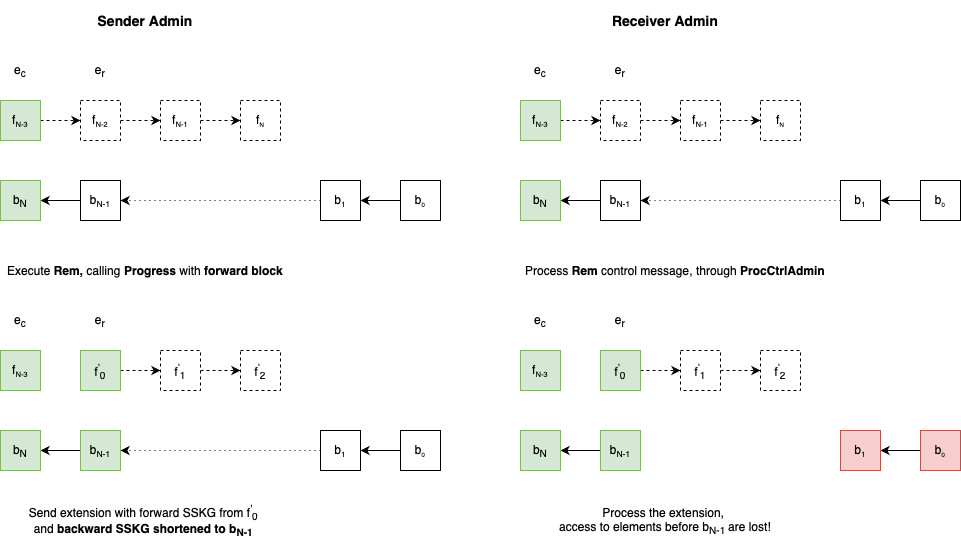
\includegraphics[width=1\textwidth]{figures/bug1.png}
    \caption{Example of DKR admin state loss after processing an extension, as described in the first bug and its fix. 
    Note that \texttt{Rem} only starts a new forward chain.
    The green boxes represent elements of the internal chains which were released in current or previous epochs. 
    Boxes with solid borders represent the state that the admin stores or has already materialized at least once.
    Dashed boxes and lines represent derivable elements from current state.
    Red boxes describe elements that were stored / accessible but are lost in the current epoch.
    Note that at epoch $e_c$ the admins are synchronized having the same local view on the global state.}
    \label{fig:process-extension-fix}
\end{figure}

\paragraph{Bug 1:} The admin operations \texttt{Rem}, \texttt{RemAdm} and
\texttt{RotKeys} require to advance the DKR state from the current epoch
$e_{c}$
to the next epoch $e_{r}$ and add blocks, meaning that new chains are created, 
either a forward, backward or both.
When an admin receives messages containing such operations and related
state updates, it will execute the \texttt{ProcCtrlAdmin} procedure.
In this procedure, the receiver admin will reconcile the local DKR state
with the state update received from the sender admin.
We note that the receiving admin at the time of receiving the message
has its local state synced up to epoch $e_{c}$.
While the \texttt{RemAdm} and \texttt{RotKeys} operations are sending 
the full DKR state, \texttt{Rem} is just sending an extension of the current state. 
This extension was however ignored by the receiving admin, 
which would just get out of sync. We adjusted the \texttt{ProcCtrlAdmin}
procedure to also handle the case where an extension is sent,
and process it. To this end, the receiving admin calculates the
interval of its complete local DKR state, from epoch 0 to the current
local epoch $e_c$. Then it will extend the interval with the extension
received from the sender admin, thus having access to the state up to
the epoch $e_r$. Finally, the resulting interval is used to override the
local DKR state of the admin. 
Notice that the sender admin might still
have access to a bigger state than the receivers,
as receiving admins are forced to shorten their last backward chain
to epoch $e_r$ to correctly process the extension.
However, the admin group will still be able to progress forward
to a new epoch $e_{r+1}$, and maintain all the local views of the DKR state
synchronized. We distinguish two cases, depending on which admin is
executing the next operation:

\begin{itemize}
    \item If the next operation is performed by the same sender admin,
the state of all other admins will be updated with a new extension or with
a full state update, depending on the operation.

\item When the next operation is performed by a different sender admin,
then a new backward chain will be started. The new initial element will 
be sent in the extension and the admin still holding the larger state
will also shrink its state to the epoch $e_r$. 
Then the extension will be processed, so the new initial element
will be added to start a new backward chain, and the state will be
synchronized up to epoch $e_{r+1}$. All other receiving admins will
also process the extension and will be able to progress to the new epoch,
following the same procedure, with the detail that the last backward chain
has already been shortened to epoch $e_r$ in the previous operation.

\end{itemize}

The implications of this na\"ive approach, where admins use the same
mechanism of members to extend their local state, is that in case admins
alternate in performing operations, at each operation a new backward chain
will be started, resulting in an average space complexity of $O(n)$ 
for the initial elements.
Another possible solution would be to send the DKR state also
in case of a \texttt{Rem} operation. This would instead 
increase the bandwidth usage.

\paragraph{Bug 2:} The second bug is caused by an optimization,
with which admins spare on the bandwidth usage while sending the new DKR state
from a sender admin to receiver admins.
An admin performing the \texttt{Add}, \texttt{UpdAdm} or \texttt{AddAdm} operations needs to advance the global epoch of the group and only release a new forward chain element.
This is performed by calling the \texttt{progress} procedure on the current
DKR state. No block is needed, as we only need to disallow
the new member of the group from generating keys corresponding
to epochs before the one in which he joined. Therefore, the receiving
admins would need only to call progress on their local copy of the DKR
global state and should be able to calculate the new forward chain element.
However, recalling the generalisation of the DKR construction,
we might be exactly at the epoch corresponding to a maximum chain length,
either for the latest forward chain, the latest backward chain or both.
In this case, the sender admin would need to generate a new random initial 
element for the new chain(s). If also the receivers randomly sample new 
initial elements in their local state, all admins would be out of sync.
The fix we have implemented is to also send an extension in those cases,
with the same implications as seen above for the other bug.


\subsection{DKR enhancements}\label{sc:DKR-enhancements}

In the discussion on the implications of the adjustments to GRaPPA in ~\cref{sc:GRaPPA-bugs},
we have seen how the admins can get out of sync.
We highlight that the current na\"ive solution still
has some drawbacks, as the state of all admins is not
fully synchronized, where an admin maintains a larger state
comprising all the latest backward chain elements other admins
lost access to.

The key point we want to stress is that the DKR primitive
does not capture the distinction between a full DKR state,
with read/write access, and a partial DKR state, with read-only access
together with the associated operations.
We claim that this distinction is crucial to understanding the discrepancy existing between the state of two clients with different capabilities,
namely admins and members, and provide a more detailed specification
of the two compared to the one provided in the original manuscript of \cite{GKP} (\cref{sc:background-generalised-DKR}):

\begin{itemize}
    \item A DKR full state, which we will simply call DKR state,
    comprises: 
    the current epoch $e_{max}$, 
    the complete list of backward chains
    and the complete list of forward chains,
    from epoch $0$ to epoch $e_{max}$ and 
    a parameter $N$ indicating the maximum length of a chain.
    Each chain is stored from its initial element. 
    In particular, the latest backward chain
    is stored from the initial element of the element sequence order,
    which corresponds to the latest possible element which will be released.
    The state thus contains all the elements to derive the state up to
    the current $e_{max}$ epoch and possibly beyond. 
    In case the latest forward chain is not fully used, i.e.,
    the latest $N$-element was not yet released, and the backward
    chain is not also fully used, i.e., the element
    corresponding to $e_{max}$ is not the initial element of the chain,
    it is possible to compute new elements of both
    chains, which can be used to derive keys for the next epochs.
    \item An interval state is a subset of the DKR state, which
    allows deriving keys for the epochs represented in the interval.
    It comprises: the epoch interval with the starting ($e_{left}$) and ending ($e_{right}$) 
    epochs, with the constraint $0 \leq e_{left} \leq e_{right} \leq e_{max}$,
    where $e_{max}$ is the current epoch of the DKR state from which the interval
    state is extracted. Also, it includes the slices of the backward
    and forward chains corresponding to the epochs in the interval.
    More precisely, the forward (respectively backward) chain from which the
    element for the epoch $e_{left}$ (respectively $e_{right}$) can be derived
    is shrunk to that element, disallowing the derivation of any key outside the epoch interval.
\end{itemize}

When we consider a shared DKR state among multiple clients,
as in the implementation of GRaPPA, it becomes clear
that an operation to extend a copy of the DKR state is
missing in the scheme.
We therefore propose to add the following operation to the DKR
primitive, of which we provide an informal description:

\begin{itemize}
    \item \texttt{CreateFExt($st$, $l$)}, on input the DKR state $st$ and an epoch $l$,
    returns a full-extension $fext$ or error. The full-extension is an interval state
    starting at epoch $l$ and ending at the current $e_{max}$ epoch of the DKR state
    $st$, similarly to an extension. However, in a full extension, we do not 
    specify the ending epoch, as the latest backward chain included in the interval
    could give access to state beyond the current epoch. Practically speaking,
    the full extension is an extension where the latest backward chain is not shrunk.
    We further highlight that full extensions always comprise the latest current epoch,
    as they serve the specific purpose of extending the state of a replica of the DKR state.
    Also, a full extension contains the current epoch $e_{max}$.

    \item \texttt{ProcessFExt($st$, $fext$)}, on input the DKR state $st$ and a full-extension $fext$,
    returns the updated DKR state $st'$ or error. The procedure processes the full-extension
    $fext$ on the provided $st$ as the existing \texttt{ProcExt} operation processes an extension $ext$
    on a provided interval state $int$, with the additional
    operation of setting the state current epoch $st.e_{max}$ to the current epoch contained
    in the full-extension $fext.e_{max}$.
    
\end{itemize}

\paragraph{Solving the Bugs in GRaPPA}
Equipped with the new full-extension entity, its creation and processing operations,
the enhanced DKR primitive can be now used in the GKP instantiation
GRaPPA to solve the bugs from \cref{sc:GRaPPA-bugs}.
Instead of applying the na\"ive solution, where the admins extend their local state as members, or they always send each other the full state, the admins can now send full extensions among them for all operations that require progressing the DKR state,
i.e.\ all admin operations.
This will allow them to keep their local copy of
the DKR state synchronized, with an optimal constant bandwidth 
consumption, thus serving the purpose of correcting the 
protocol and clarify how to minimize bandwidth consumption.

%\paragraph{Optimise Transactional Storage of DKR}

%With the new operations \texttt{CreateFExt} and \texttt{ProcessFExt},
%we can optimise the transaction storage of the DKR state in a client.
%This use case is not only present inside GRaPPA, but in any practical
%usage of DKR alone. However, a related discussion can be found in \cref{sc:state-sync-rollbacks}.

%Let's imagine the case in which a client 
